\section{Energy integration}


Nasibeh use cetow for heat puming solutions and st fons for large scale integration and combined heat and power production. We have to use neutralised values (i.e. we start with 100 unit and end up with 46.


Converting energy resources into useful energy, exergy efficiency, heat pumping and combined heat and power => examples from the papers of Nasibeh

adding a citation \cite{Pouransari_2014}

testing equations
\begin{equation}
min \, obj= \frac{things_{good}}{things_{bad}} \forall things\\
\text{subject to}  \\
things_{bad}\ge necessary\,\, level \cup unnecessary \, level
\end{equation}

**************

\subsection{Caste study I: Energy integration technologies}

The process heat transfer requirement for a real chemical site is identified using the data collected from different sources including energy conversion, distribution or process units. The heating and cooling requirements have been consequently determined.Based on the heating and cooling requirement definition, the Composite and the Grand Composite Curves are generated in \cref{fig1:mer}. It should be noticed that while defining the energy requirements, we have introduced the streams with the highest possible degree of freedom in order to target the greatest scope for improvement. An individual $\Delta T_{min}$ contribution is considered for each stream by adopting the typical value calculated from a predefined heat exchanger with the film heat transfer coefficient of each fluid at its relevant physical state. The Maximum Energy Recovery (MER) is then determined for the given $\Delta T_{min}$ and is considered as an initial target for heat recovery. \cref{fig1:mer}a shows the maximum heat recovery, the hot and the cold MER. In this case, there is a 54\% potential of integration (from the total heating requirement) compared to 40\% of integration in the current process which corresponds to the first ideal target.


        \begin{figure}[h]
        \begin{center}
        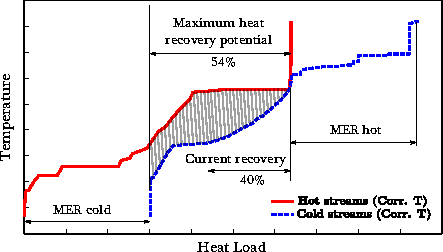
\includegraphics [height=4.3cm]{figures/EnergyIntegration/figMERcc.pdf} 
        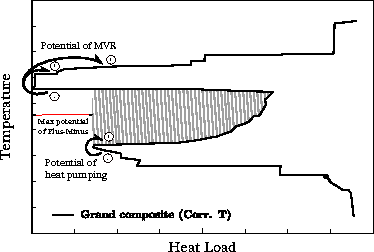
\includegraphics [height=4.3cm]{figures/EnergyIntegration/figMERgcc.pdf}
        \caption{Composite and Grand Composite Curves of the process after heat integration}
        \label{fig1:mer}
        \end{center}
        \end{figure}
        



      \begin{figure}[h]
      \begin{center}
      \begin{tabular}{cc}
        \subfloat[With MVR]{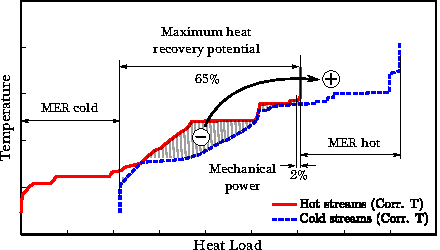
\includegraphics [height=4cm]{figures/EnergyIntegration/HPmvr_mvralone.pdf}} & 
        \subfloat[With MVR and HP]{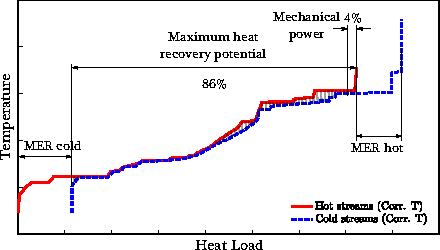
\includegraphics [height=4cm]{figures/EnergyIntegration/HPmvr_mvrhp.pdf}}
       \end{tabular}
      \caption{Composite Curves after improvement potentials}
      \label{fig1:HPmvr}
      \end{center}
      \end{figure}
